\documentclass[11pt]{article}

\usepackage[margin=1in]{geometry}
\usepackage{setspace}
\usepackage{graphicx}
\usepackage{booktabs}
\usepackage{float}
\usepackage{placeins}
\usepackage{hyperref}
\usepackage{enumitem}
\usepackage{parskip}
\usepackage[T1]{fontenc}
\usepackage{lmodern}
\usepackage[authoryear,round]{natbib}

\hypersetup{
    colorlinks=true,
    linkcolor=black,
    citecolor=black,
    urlcolor=blue
}

\setstretch{1.15}
\setlength{\parindent}{0pt}
\raggedbottom
\setlength{\textfloatsep}{10pt plus 2pt minus 2pt}
\setlength{\floatsep}{10pt plus 2pt minus 2pt}
\setlength{\intextsep}{10pt plus 2pt minus 2pt}
\setlength{\abovecaptionskip}{5pt}
\setlength{\belowcaptionskip}{0pt}

\title{\textbf{Module 6 Assignment: Otomoto Marketing Segmentation Model Optimization}}
\author{
Emmanuel Fru\\
BAN6440 -- Machine Learning\\
Professor: Dr. Preethi Natarajan\\
Nexford University
}
\date{September 13, 2026}

\begin{document}

\maketitle

\section{Business Context and Problem Framing}

The assignment presents the task as optimizing an artificial neural network used by Otomoto for marketing segmentation. However, the supplied dataset does not contain automotive customers or marketing segment labels. It contains 7,043 telecommunications customer records covering account tenure, subscribed services, contract type, billing method, monthly charges, total charges, and whether the customer churned.

For this reason, I treated the dataset as a supervised customer churn classification problem. This still supports the marketing objective of the assignment. Customers identified as having a higher probability of churn can be targeted with retention campaigns, while lower-risk customers can be handled differently. Churn prediction is widely used in telecommunications because identifying customers at risk of leaving can support more focused retention activity \citep{vafeiadis2015,ahmad2019,amin2019}.

The target variable is moderately imbalanced. Of the 7,043 customers, 5,174 did not churn and 1,869 did. This means 73.46\% of customers belong to the majority class. A model that predicted ``No Churn'' for every customer would therefore achieve 73.46\% accuracy without learning anything useful. I used this as the minimum accuracy benchmark when evaluating the ANN.

The objective of the optimization was to determine whether optimizer choice could improve the performance of the ANN. Adam, RMSprop, and stochastic gradient descent (SGD) were compared while keeping the dataset, ANN architecture, preprocessing, batch size, loss function, and early stopping conditions fixed. Each optimizer was run across five random seeds to reduce the influence of a single favourable or unfavourable training run.

F1-score for the churn class was used as the primary selection metric, with recall as the first tie-breaker. Recall matters because failing to identify a customer who is likely to churn can result in a missed retention opportunity. Precision also matters because incorrectly flagging too many customers would increase the cost of the marketing campaign.

\section{Existing ANN and Baseline Assessment}

I first recreated the ANN logic supplied with the assignment so that there was a clear ``before optimization'' result. The existing workflow label-encoded categorical variables, dropped the 11 rows where \texttt{TotalCharges} was blank, used a 75/25 train-test split, applied SMOTE to the training data, and trained an Adam-based neural network for five epochs. SMOTE creates synthetic minority-class observations to reduce class imbalance \citep{chawla2002}.

The recreated network contained 19 input features followed by hidden layers of 19, 15, and 10 neurons, all using ReLU activation, and a single sigmoid output for binary classification. Its loss function was binary cross-entropy.

\begin{center}
\begin{tabular}{c}
\textbf{19 input features}\\
$\downarrow$\\
Dense(19, ReLU)\\
$\downarrow$\\
Dense(15, ReLU)\\
$\downarrow$\\
Dense(10, ReLU)\\
$\downarrow$\\
Dense(1, Sigmoid)
\end{tabular}
\end{center}

The legacy model produced the results in Table~\ref{tab:legacy}.

\begin{table}[H]
\centering
\caption{Recreated legacy ANN results}
\label{tab:legacy}
\begin{tabular}{lr}
\toprule
\textbf{Metric} & \textbf{Result}\\
\midrule
Accuracy & 56.9\%\\
Precision & 37.0\%\\
Recall & 88.7\%\\
F1-score & 52.2\%\\
ROC-AUC & 74.4\%\\
True negatives & 586\\
False positives & 705\\
False negatives & 53\\
True positives & 414\\
\bottomrule
\end{tabular}
\end{table}

The model's main strength was recall. It identified 414 of 467 churners in its test split. However, the overall model was not suitable for an efficient retention campaign. Its 56.9\% accuracy was below the 73.5\% majority-class benchmark. Precision was only 37.0\%, and 705 non-churners were incorrectly classified as churn risks. This means the model caught many genuine churners by also flagging a very large number of customers who were not going to leave.

The baseline also had methodological weaknesses. Label encoding gives categorical values arbitrary integer relationships that do not necessarily represent the meaning of the categories. The numeric variables were not standardised. The 11 blank \texttt{TotalCharges} records were removed even though all 11 belonged to customers with zero tenure. The supplied workflow also used the test split during training as validation data. I treated these issues as part of the model optimization problem rather than attributing all improvement to optimizer choice alone.

\section{Data Preparation and Revised ANN}

\subsection{Data Cleaning}

The raw dataset contained 7,043 rows and 21 columns. There were no duplicate rows and no duplicate customer IDs. Pandas initially reported no missing values, but inspection of \texttt{TotalCharges} identified 11 blank strings. All 11 occurred where \texttt{tenure = 0}. I converted \texttt{TotalCharges} to numeric and assigned these records a value of 0 rather than deleting the customers. This retained all 7,043 observations.

The \texttt{customerID} field was removed because it is an identifier rather than a predictive feature. The target variable was encoded as:

\begin{itemize}[leftmargin=*]
    \item Churn = Yes $\rightarrow$ 1
    \item Churn = No $\rightarrow$ 0
\end{itemize}

The remaining dataset contained 19 raw predictors.

\subsection{Encoding, Scaling, and Data Split}

The categorical predictors were transformed using one-hot encoding with the first category dropped and unknown categories ignored. One-hot encoding represents categories as binary indicator variables rather than imposing an artificial numerical order \citep{sklearnOHE}. After transformation, the ANN received 30 input features.

The numeric variables were:

\begin{itemize}[leftmargin=*]
    \item \texttt{SeniorCitizen}
    \item \texttt{tenure}
    \item \texttt{MonthlyCharges}
    \item \texttt{TotalCharges}
\end{itemize}

These variables operate on different scales, especially \texttt{TotalCharges} compared with the binary \texttt{SeniorCitizen} field. I therefore used \texttt{StandardScaler}. The scaler and encoder were fitted on the training split only, then applied to the validation and test sets. This avoids using held-out data statistics during training, which would create data leakage \citep{sklearnScale}.

The cleaned data was split using stratification and \texttt{random\_state=42}:

\begin{table}[H]
\centering
\caption{Final data split}
\label{tab:splits}
\begin{tabular}{lrrr}
\toprule
\textbf{Split} & \textbf{Rows} & \textbf{Churn} & \textbf{Churn Rate}\\
\midrule
Training & 4,930 & 1,308 & 26.53\%\\
Validation & 1,056 & 280 & 26.52\%\\
Test & 1,057 & 281 & 26.58\%\\
\bottomrule
\end{tabular}
\end{table}

The numeric training features had means effectively equal to zero and standard deviations effectively equal to one after scaling. The similar churn rates across all three splits confirmed that stratification worked as intended.

\subsection{Revised ANN Architecture}

For the controlled optimizer experiment, I used one fixed ANN architecture for all three optimizers:

\begin{center}
\begin{tabular}{c}
\textbf{30 encoded input features}\\
$\downarrow$\\
Dense(32, ReLU)\\
$\downarrow$\\
Dropout(0.30)\\
$\downarrow$\\
Dense(16, ReLU)\\
$\downarrow$\\
Dense(1, Sigmoid)
\end{tabular}
\end{center}

The revised architecture is small enough for a dataset of this size while providing more capacity than the original model to work with the expanded one-hot encoded feature space. Dropout was included as regularisation. The loss function remained binary cross-entropy.

This means the before-and-after comparison is a comparison of the supplied legacy workflow against the complete revised pipeline. It should not be interpreted as evidence that optimizer choice alone produced the full performance difference. To isolate optimizer effects, Adam, RMSprop, and SGD were compared only within the revised pipeline using the same architecture and data split.

\section{Optimization Methodology}

\subsection{Optimizer Selection}

I compared three optimizers named directly in the assignment and commonly used for neural-network training:

\begin{itemize}[leftmargin=*]
    \item \textbf{Adam}, with learning rate 0.001
    \item \textbf{RMSprop}, with learning rate 0.001
    \item \textbf{SGD}, with learning rate 0.01
\end{itemize}

Adam adapts updates using estimates of the first and second moments of the gradients \citep{kingma2015,tfAdam}. RMSprop scales updates using a moving average of squared gradients \citep{tfRMSprop}. SGD applies gradient-based weight updates directly and used the larger learning rate of 0.01 in this experiment \citep{tfSGD}.

The learning rates were declared explicitly rather than relying on hidden defaults. The larger SGD learning rate was intentional because plain SGD generally uses a larger update step than Adam and RMSprop. The goal was to compare reasonable optimizer configurations, not to force every algorithm to use the same numerical learning rate.

\subsection{Controlled Experiment Design}

Each optimizer used exactly the same:

\begin{itemize}[leftmargin=*]
    \item training, validation, and test split;
    \item ANN architecture;
    \item binary cross-entropy loss;
    \item batch size of 32;
    \item maximum of 150 epochs;
    \item dropout rate of 0.30;
    \item validation-loss early stopping with patience of 10;
    \item classification threshold of 0.50.
\end{itemize}

TensorFlow's early stopping callback can stop training when the monitored validation metric stops improving and restore the best weights \citep{tfEarlyStopping}.

Neural-network training is stochastic, so a single training run can give a misleading comparison. I therefore trained every optimizer across five seeds: 42, 123, 456, 789, and 2026. This produced 15 validation experiments. The customer split remained fixed at \texttt{random\_state=42}; only the network initialization and training randomness changed.

The final optimizer was selected using validation data only. The decision rule was defined before the test set was evaluated:

\begin{enumerate}[leftmargin=*]
    \item highest mean validation F1-score;
    \item highest mean recall if F1 was tied;
    \item highest mean precision if the first two metrics were tied.
\end{enumerate}

This approach is consistent with prior churn research that evaluates multiple classification metrics rather than relying on accuracy alone \citep{vafeiadis2015,amin2019}.

\section{Optimizer Comparison Results}

Table~\ref{tab:optimizers} reports mean and standard deviation across the five seeds.

\begin{table}[H]
\centering
\caption{Validation performance across five random seeds}
\label{tab:optimizers}
\small
\begin{tabular}{lrrrrrr}
\toprule
\textbf{Optimizer} & \textbf{Accuracy} & \textbf{Precision} & \textbf{Recall} & \textbf{F1} & \textbf{ROC-AUC} & \textbf{Epochs}\\
\midrule
Adam & .802 $\pm$ .006 & .648 $\pm$ .024 & .564 $\pm$ .027 & .602 $\pm$ .008 & .846 $\pm$ .002 & 31.8 $\pm$ 5.3\\
RMSprop & .801 $\pm$ .006 & .647 $\pm$ .021 & .550 $\pm$ .027 & .594 $\pm$ .012 & .843 $\pm$ .001 & 33.6 $\pm$ 7.8\\
SGD & \textbf{.804 $\pm$ .002} & .648 $\pm$ .010 & \textbf{.576 $\pm$ .032} & \textbf{.609 $\pm$ .014} & .845 $\pm$ .001 & 97.6 $\pm$ 32.4\\
\bottomrule
\end{tabular}
\end{table}

SGD achieved the highest mean validation F1-score at 0.609 and the highest mean recall at 0.576. It was therefore selected under the predefined decision rule. However, the result needs qualification. SGD's mean F1 advantage over Adam was only 0.007, which is small relative to the observed run-to-run variation. Adam also converged much faster, averaging 31.8 epochs compared with 97.6 for SGD, and its F1-score was more stable across seeds.

RMSprop did not provide a clear advantage. Its mean F1, recall, accuracy, and ROC-AUC were slightly below the other two configurations.

The optimizer comparison therefore produced two different conclusions. SGD was the nominal performance winner under the predefined rule. Adam was the more computationally efficient alternative. The difference between them was not large enough to argue that SGD is universally superior for this dataset.

\begin{figure}[!htbp]
\centering
\IfFileExists{outputs/optimizer_f1_comparison.png}{
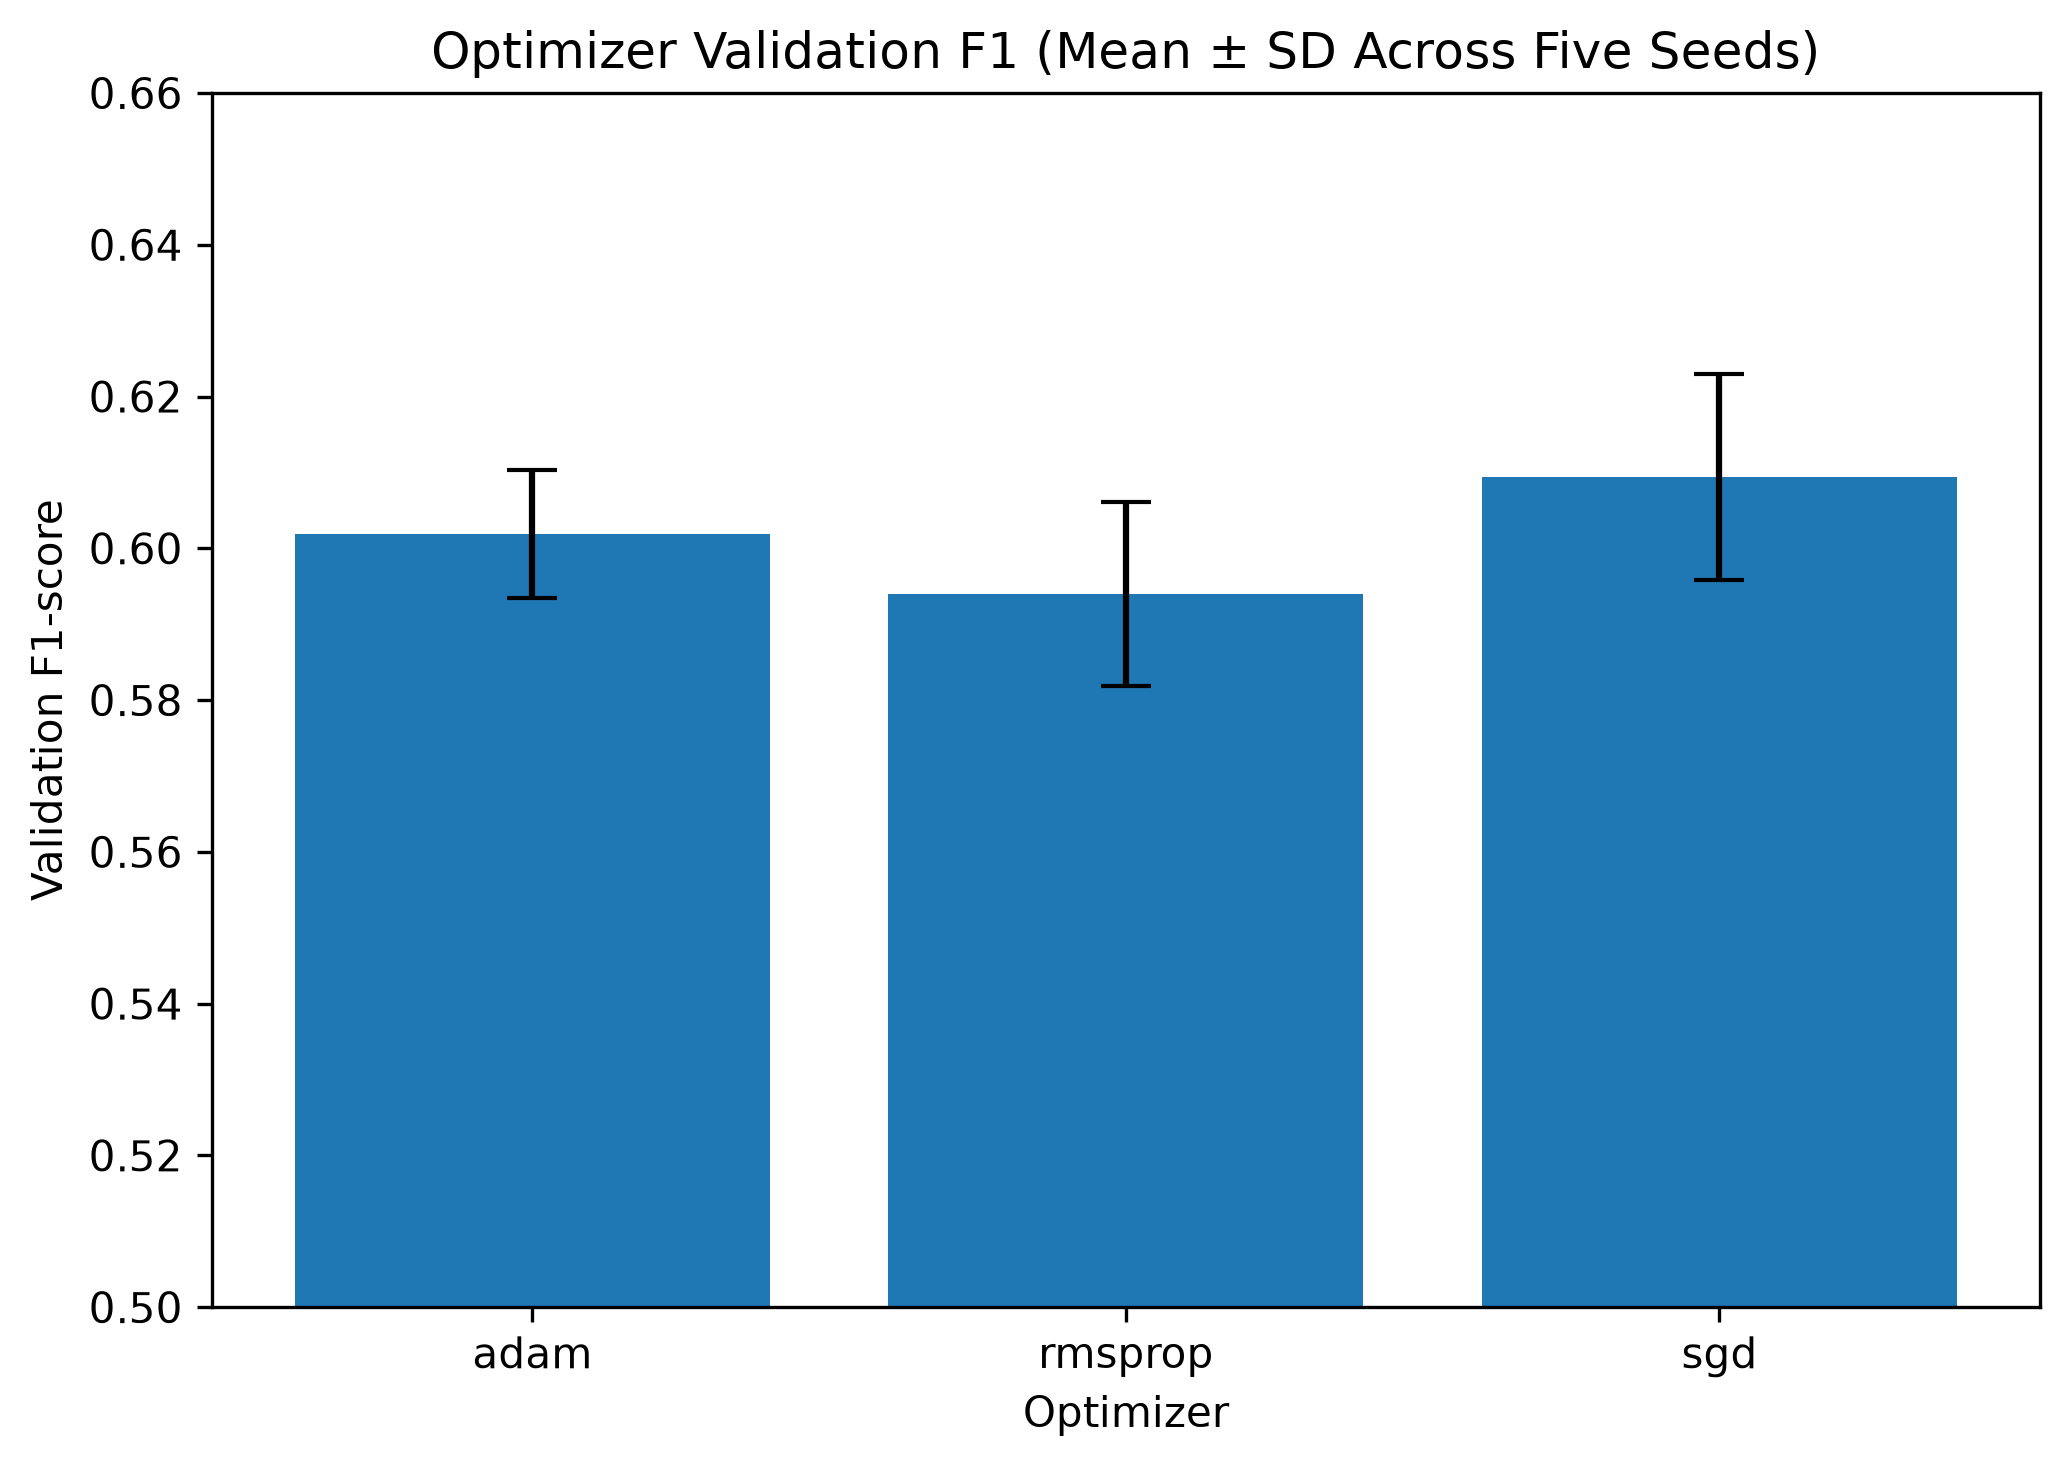
\includegraphics[width=0.68\textwidth]{outputs/optimizer_f1_comparison.png}
\caption{Validation F1-score by optimizer, reported as mean and standard deviation across five seeds.}
}{
\fbox{\parbox[c][2in][c]{0.82\textwidth}{\centering Missing: \texttt{outputs/optimizer\_f1\_comparison.png}}}
}
\end{figure}

\begin{figure}[!htbp]
\centering
\IfFileExists{outputs/optimizer_epochs_comparison.png}{
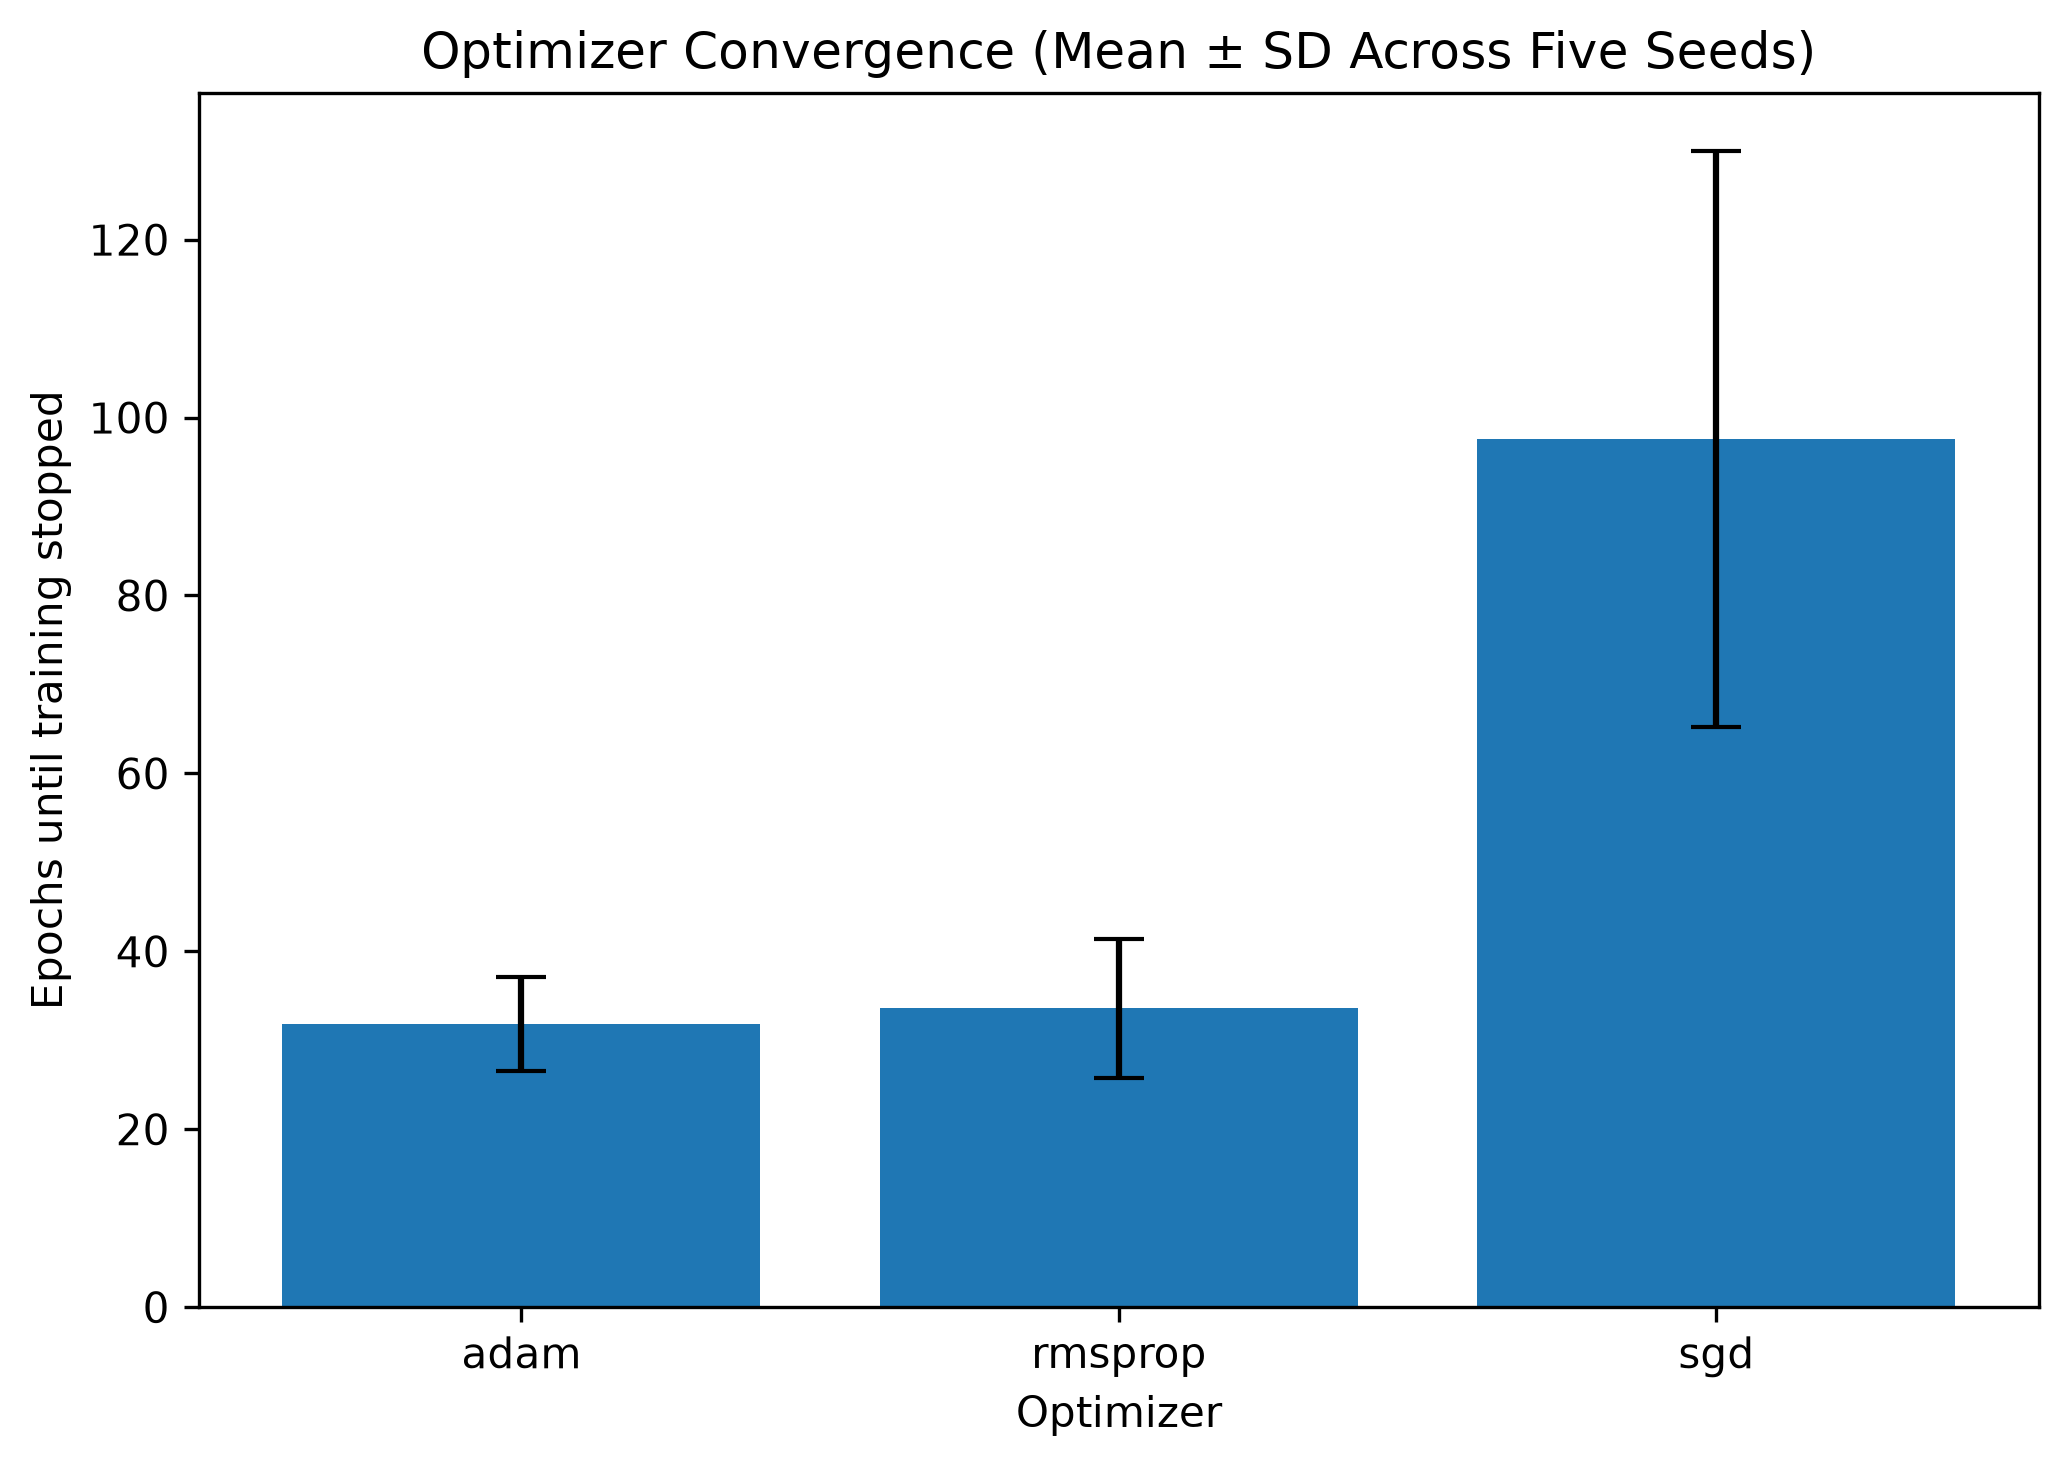
\includegraphics[width=0.68\textwidth]{outputs/optimizer_epochs_comparison.png}
\caption{Average number of training epochs by optimizer.}
}{
\fbox{\parbox[c][2in][c]{0.82\textwidth}{\centering Missing: \texttt{outputs/optimizer\_epochs\_comparison.png}}}
}
\end{figure}

\begin{figure}[!htbp]
\centering
\IfFileExists{outputs/optimizer_loss_comparison.png}{
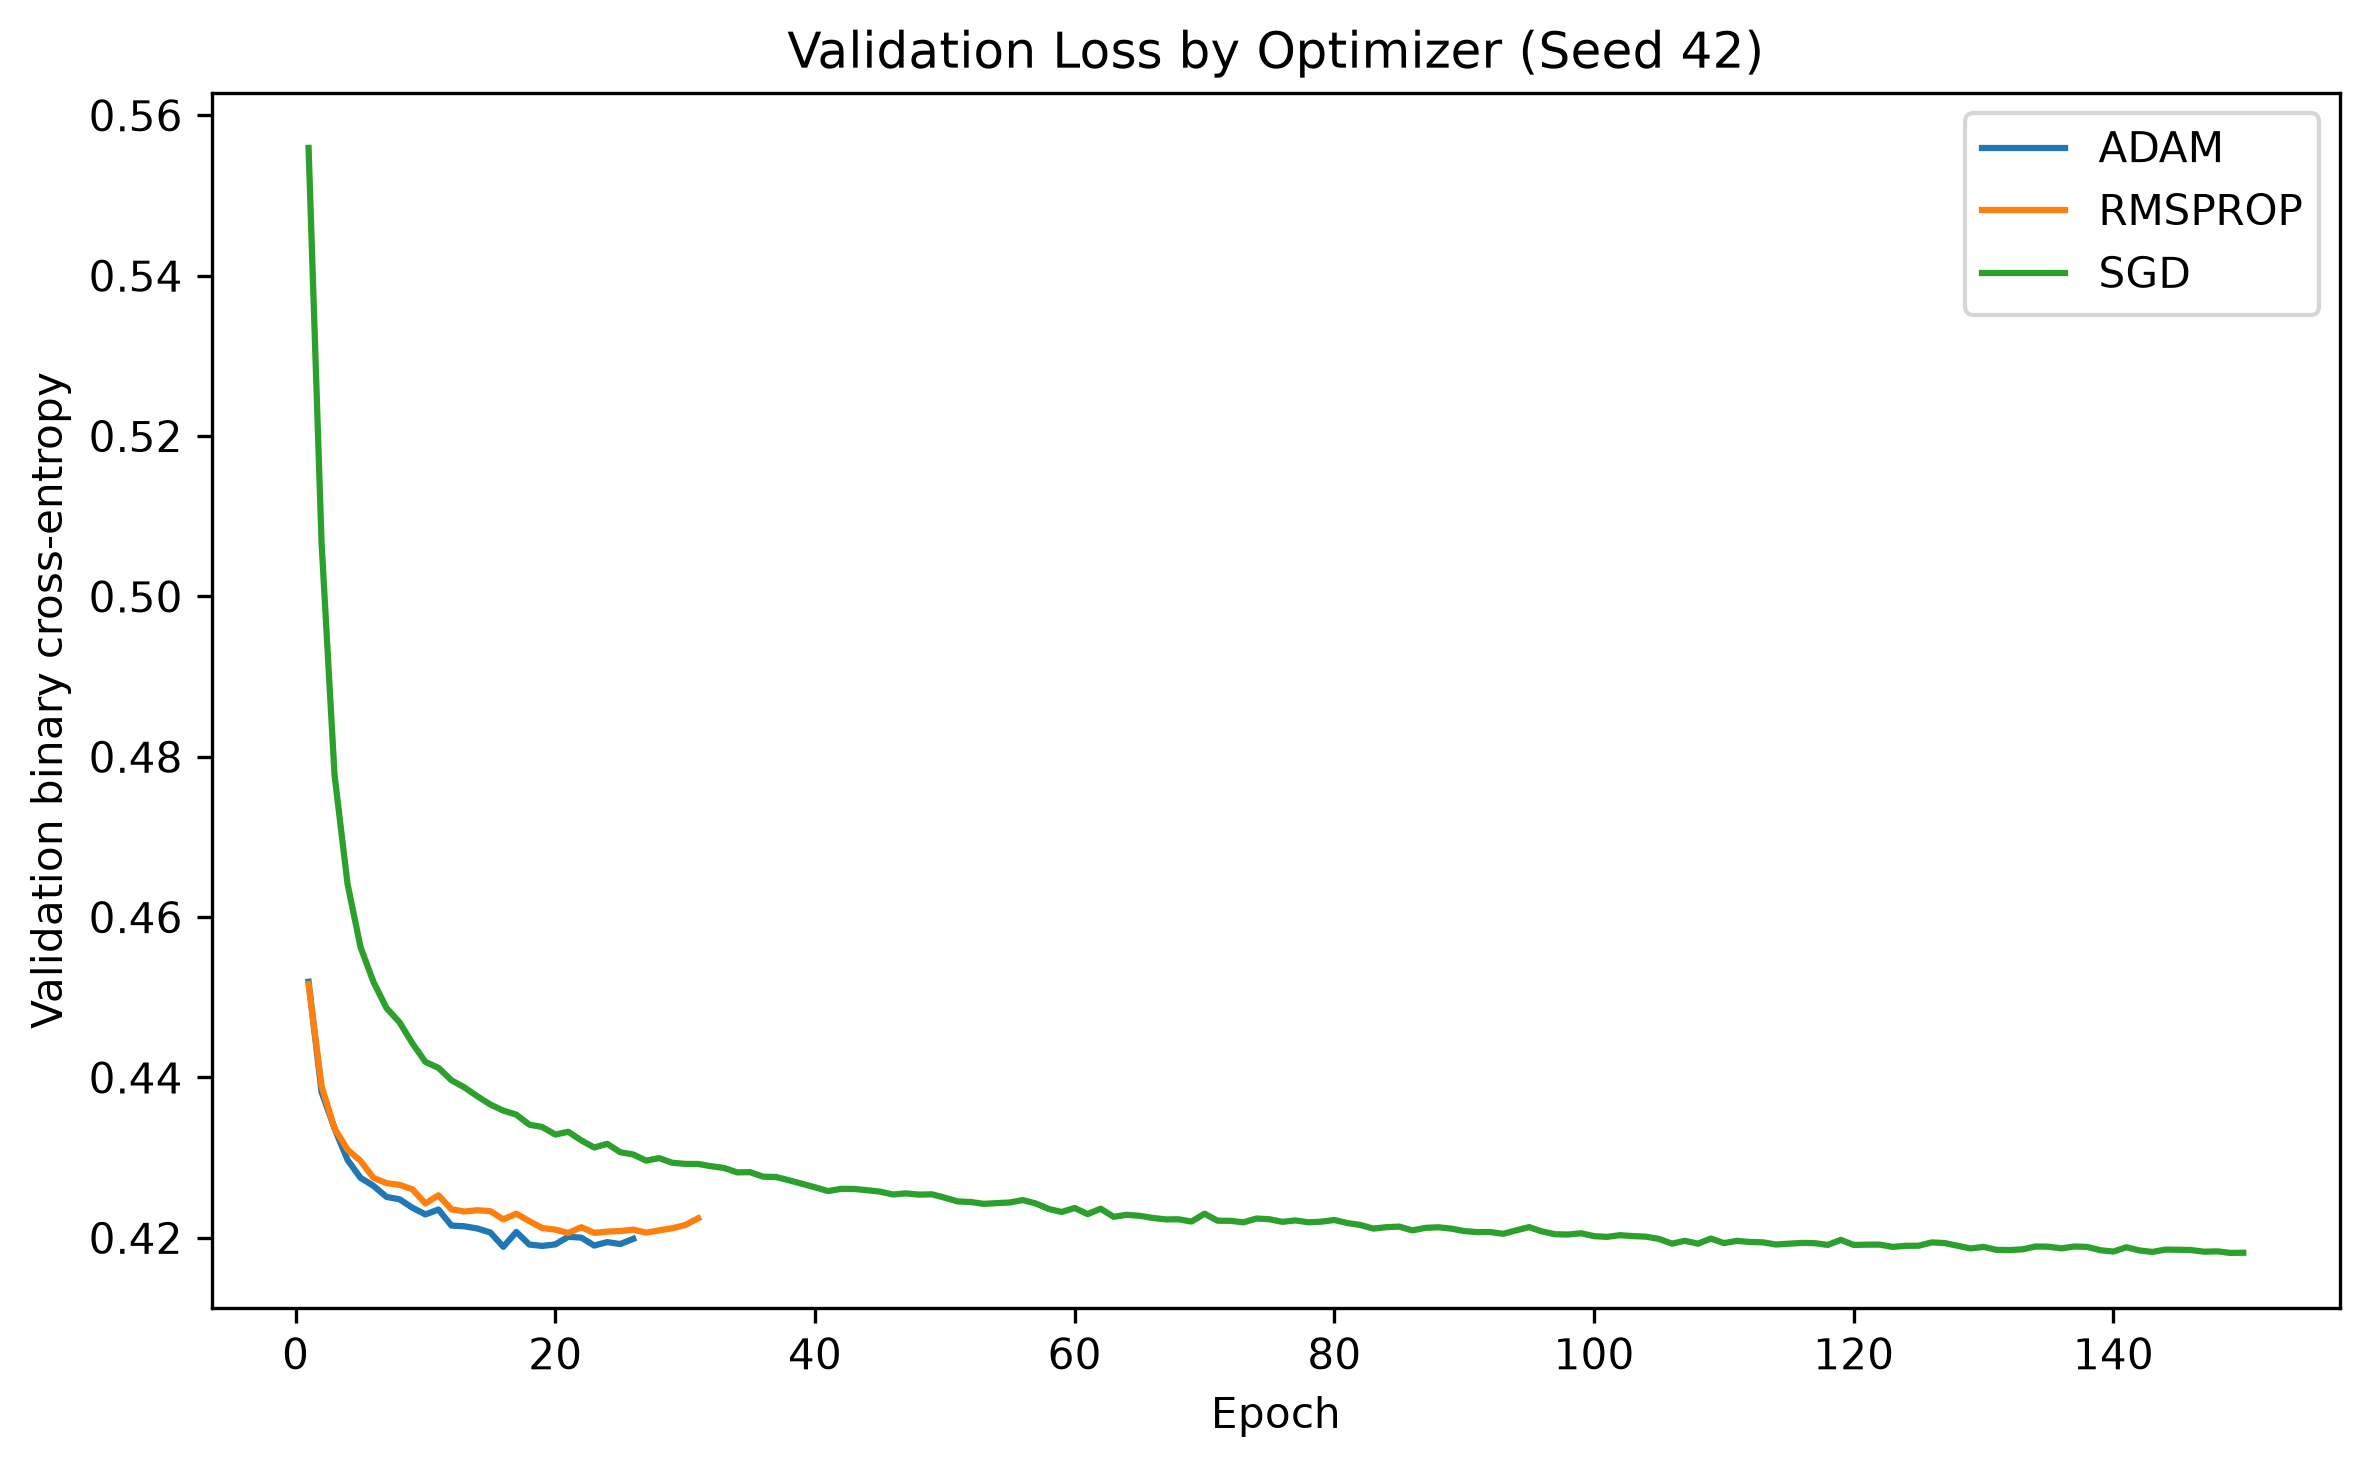
\includegraphics[width=0.72\textwidth]{outputs/optimizer_loss_comparison.png}
\caption{Representative validation-loss curves for seed 42. The seed was fixed before examining the results.}
}{
\fbox{\parbox[c][2in][c]{0.82\textwidth}{\centering Missing: \texttt{outputs/optimizer\_loss\_comparison.png}}}
}
\end{figure}

\FloatBarrier

\section{Final Model Evaluation}

After SGD was selected from validation results, I trained the fixed SGD configuration using seed 42 and evaluated the 1,057-case test set once. I did not change the optimizer, architecture, learning rate, threshold, or seed after seeing the test results.

The final training run reached the 150-epoch maximum, and the best validation-loss epoch was 149. Early stopping therefore did not terminate training before the epoch cap. This suggests that SGD convergence was still slow under the selected configuration. Because the test set had already been evaluated, I did not increase the epoch limit and retune the final model afterward. A higher epoch cap should be tested on validation data in a future experiment before evaluating new unseen test data.

\begin{table}[H]
\centering
\caption{Final held-out SGD test performance}
\label{tab:final}
\begin{tabular}{lr}
\toprule
\textbf{Metric} & \textbf{Result}\\
\midrule
Accuracy & 80.7\%\\
Precision & 69.0\%\\
Recall & 49.8\%\\
F1-score & 57.9\%\\
ROC-AUC & 84.5\%\\
True negatives & 713\\
False positives & 63\\
False negatives & 141\\
True positives & 140\\
\bottomrule
\end{tabular}
\end{table}

The majority-class accuracy on the test set was 73.4\%. The ANN therefore improved accuracy by 7.3 percentage points while also producing meaningful discrimination between churners and non-churners, with ROC-AUC of 0.845.

Of the 281 customers who actually churned, the model identified 140 and missed 141. Of the 776 customers who did not churn, only 63 were incorrectly flagged. The model predicted 203 customers as churn risks in total, which is 19.2\% of the test population. Of those 203 customers, 69.0\% were actual churners. This is much more selective than the legacy model and would allow a marketing team to focus retention activity on a smaller group.

The final metrics should still be treated as estimates. The 95\% Wilson confidence intervals were:

\begin{itemize}[leftmargin=*]
    \item Accuracy: 78.2\% to 83.0\%
    \item Precision: 62.3\% to 74.9\%
    \item Recall: 44.0\% to 55.6\%
\end{itemize}

The recall interval is especially important. The model does not identify every customer who will churn, and the point estimate should not be treated as a fixed population value.

\begin{figure}[!htbp]
\centering
\begin{minipage}[t]{0.47\textwidth}
\centering
\IfFileExists{outputs/final_confusion_matrix.png}{
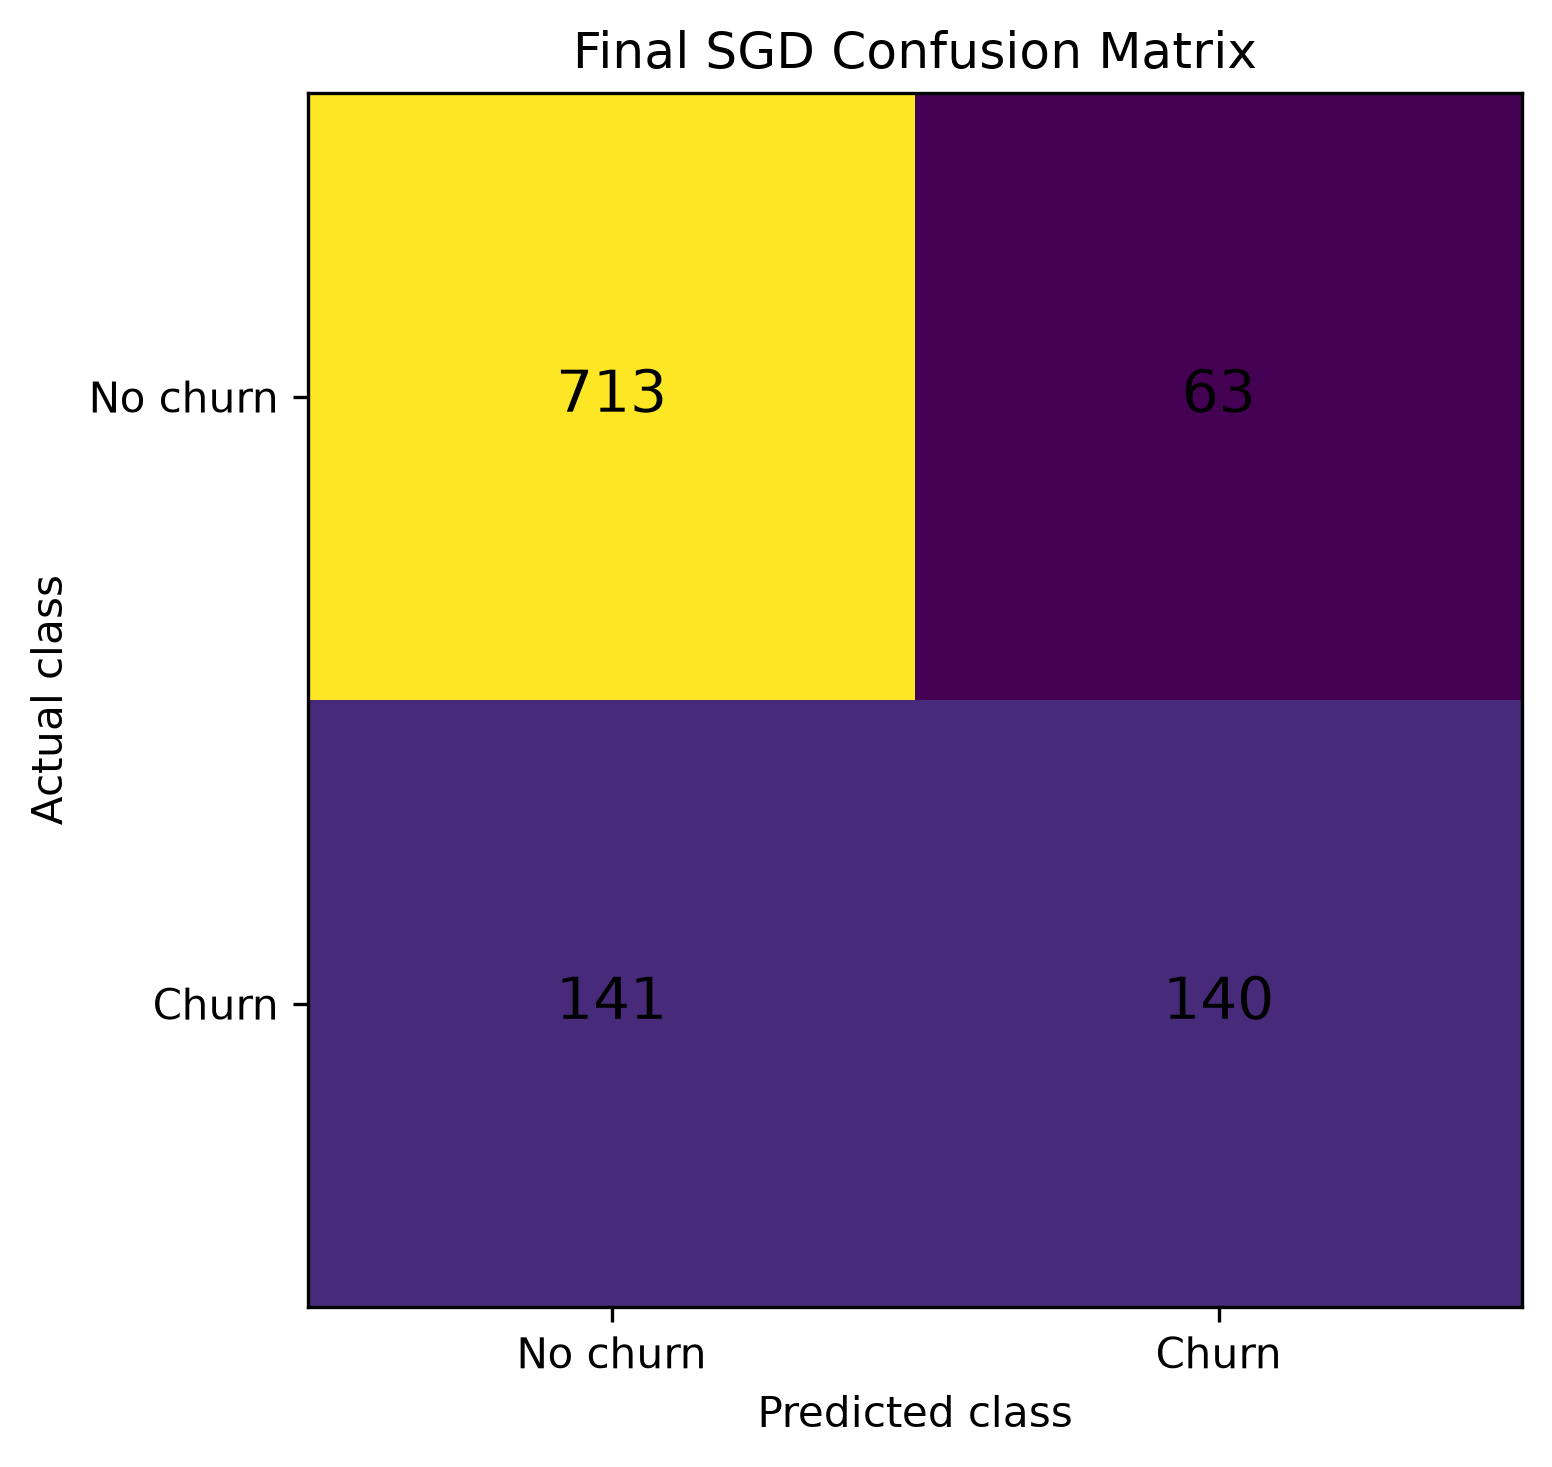
\includegraphics[width=\linewidth]{outputs/final_confusion_matrix.png}
\par\smallskip
\textbf{(a)} Final SGD confusion matrix.
}{
\fbox{\parbox[c][2in][c]{0.95\linewidth}{\centering Missing: \texttt{outputs/final\_confusion\_matrix.png}}}
}
\end{minipage}
\hfill
\begin{minipage}[t]{0.47\textwidth}
\centering
\IfFileExists{outputs/final_roc_curve.png}{
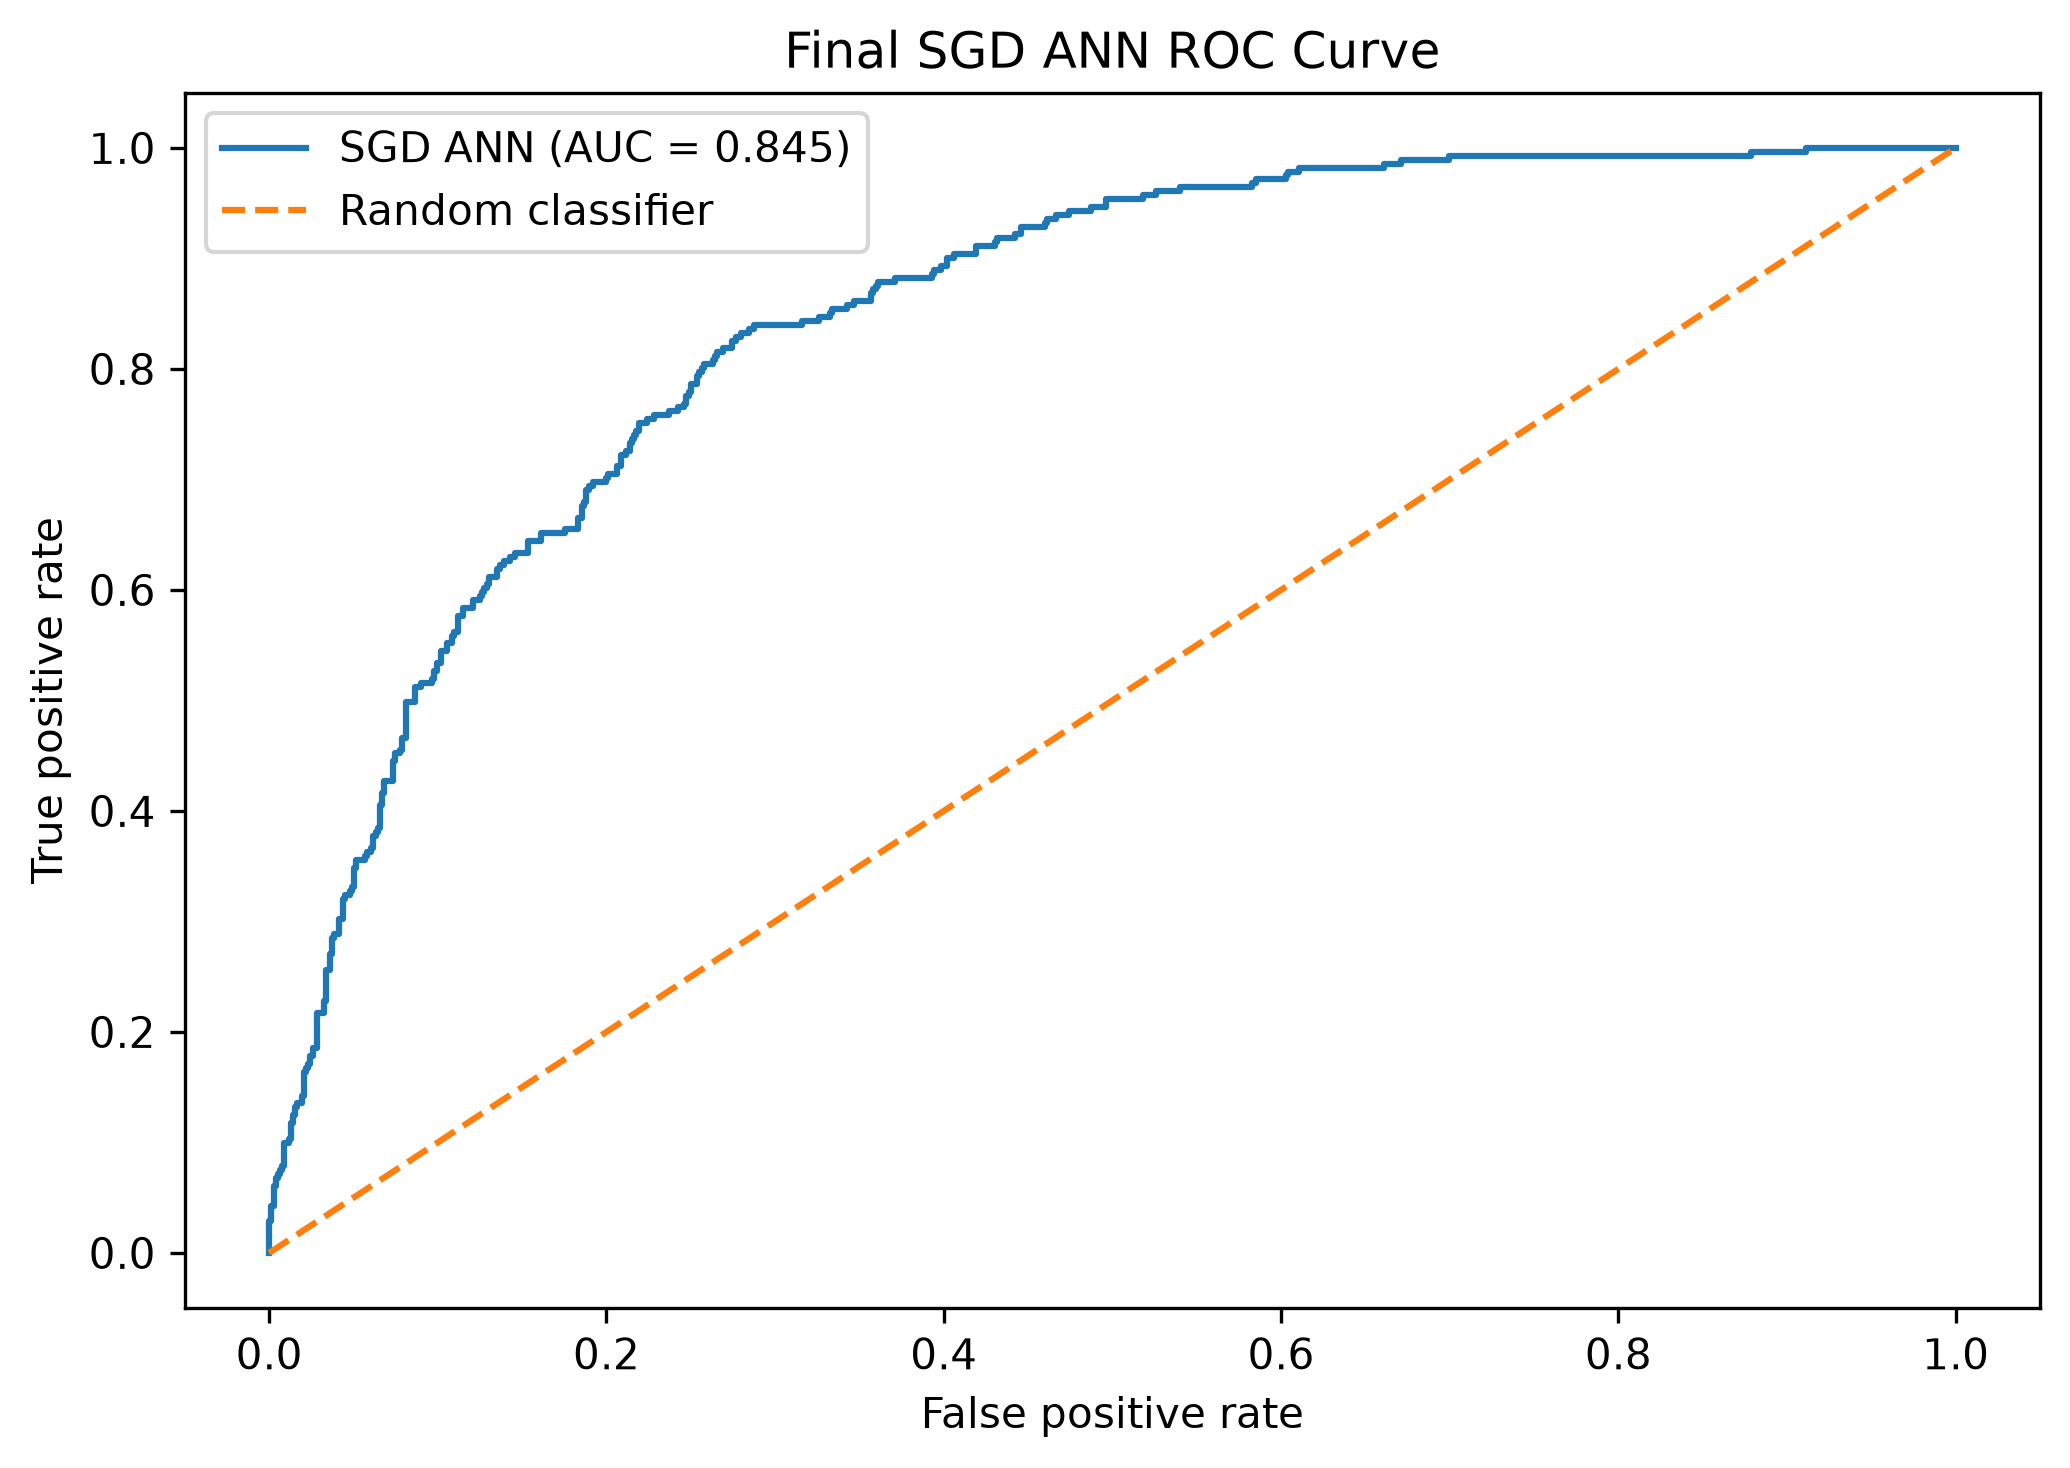
\includegraphics[width=\linewidth]{outputs/final_roc_curve.png}
\par\smallskip
\textbf{(b)} Final SGD ROC curve.
}{
\fbox{\parbox[c][2in][c]{0.95\linewidth}{\centering Missing: \texttt{outputs/final\_roc\_curve.png}}}
}
\end{minipage}
\caption{Final held-out test diagnostics.}
\end{figure}

\FloatBarrier

\section{Before and After Optimization}

Table~\ref{tab:beforeafter} compares the recreated legacy model with the final revised model.

\begin{table}[H]
\centering
\caption{Legacy model and final revised model}
\label{tab:beforeafter}
\begin{tabular}{lrr}
\toprule
\textbf{Metric} & \textbf{Legacy ANN} & \textbf{Final SGD ANN}\\
\midrule
Accuracy & 56.9\% & \textbf{80.7\%}\\
Precision & 37.0\% & \textbf{69.0\%}\\
Recall & \textbf{88.7\%} & 49.8\%\\
F1-score & 52.2\% & \textbf{57.9\%}\\
ROC-AUC & 74.4\% & \textbf{84.5\%}\\
\bottomrule
\end{tabular}
\end{table}

The revised model improved accuracy, precision, F1-score, and ROC-AUC substantially. Recall decreased. This means the final model became more selective, but it also missed more customers who eventually churned.

The legacy ANN was optimized heavily toward identifying the positive class because SMOTE balanced the training set and the model produced many positive predictions. That gave it high recall but only 37.0\% precision. A retention team using that model would contact many customers who were not actually likely to churn.

The revised model reduced this problem. Precision increased to 69.0\%, so a larger proportion of the customers flagged for intervention were genuine churners. The trade-off is that recall fell to 49.8\%. Whether that trade-off is appropriate depends on the campaign economics. If contacting customers is expensive, higher precision can be valuable. If the cost of missing a churner is much greater than the cost of an unnecessary retention offer, the decision threshold should be calibrated toward higher recall before deployment.

The two rows in Table~\ref{tab:beforeafter} were produced under different evaluation protocols, so the table should not be interpreted as a controlled optimizer-only comparison. The legacy model used a different split, SMOTE, label encoding, no numeric scaling, and a different architecture. The controlled optimizer experiment in Table~\ref{tab:optimizers} is the correct evidence for the incremental effect of Adam, RMSprop, and SGD. One of the clearest findings from the assignment is therefore that data preparation and evaluation design mattered more than the small difference between the top optimizers.

\section{Marketing Implications and Recommendations}

The final ANN can be used as a risk-ranking tool for retention campaigns rather than as a fully automated decision system. At the default 0.50 threshold, the model flagged 203 of 1,057 test customers, or 19.2\%, as churn risks. This concentrates marketing resources on a much smaller group than contacting the full customer base.

The 69.0\% precision means the flagged group is relatively focused. However, recall of 49.8\% means roughly half of the actual churners were not identified at the selected threshold. For that reason, I would not treat 0.50 as a permanent business threshold. A production campaign should select the threshold using the cost of an intervention, the value of retaining a customer, available marketing capacity, and the acceptable number of false positives.

I would recommend the following next steps:

\begin{enumerate}[leftmargin=*]
    \item Test SGD with a higher epoch cap and possibly momentum using validation data only. The final SGD run was still improving close to epoch 150.
    \item Evaluate threshold choices using campaign economics rather than a generic 0.50 cutoff.
    \item Compare the selected ANN with simpler baselines such as logistic regression and tree-based models. Previous churn studies show that different algorithms can perform well depending on the data and evaluation setup \citep{vafeiadis2015,ahmad2019}.
    \item Monitor precision, recall, churn prevalence, and calibration after deployment. Customer behaviour can change over time.
    \item Retrain only when monitoring shows meaningful deterioration or when the customer population, products, or pricing structure changes.
\end{enumerate}

\section{Challenges, Limitations, and Ethical Considerations}

\subsection{Challenges and Lessons Learned}

The first challenge was that the assignment framing did not match the supplied data. The brief described Otomoto marketing segmentation, while the file contained labelled telecom churn data. I resolved this by treating churn probability as the basis for marketing segmentation instead of forcing an unsupervised segmentation method onto a supervised target.

The second challenge was hidden data quality. \texttt{TotalCharges} appeared complete until the column was inspected as text. Eleven records contained blank strings rather than \texttt{NaN}. All 11 belonged to customers with zero tenure, so I converted them to zero instead of deleting them.

A third lesson came from the optimizer experiment. SGD had the best mean F1-score, but its advantage over Adam was small relative to the variation across seeds. A single run could easily have produced a different ranking. Running five seeds made that uncertainty visible.

The final SGD run also reached the 150-epoch cap with the best validation-loss epoch at 149. This means the early-stopping condition did not actually stop training. The result is still valid as the preselected final experiment, but it shows that convergence settings should be revisited before a future deployment.

\subsection{Methodological Limitations}

The final model has several limitations.

First, optimizer selection used five seeds but only one fixed train-validation split. Repeated stratified cross-validation would provide stronger evidence about performance across different customer samples.

Second, the final model was evaluated using one threshold of 0.50. The threshold was intentionally not changed after seeing the test set, but a production model should calibrate the operating point on validation data using business costs.

Third, the legacy and final models used different preprocessing and evaluation procedures. This means the large before-and-after improvement cannot be assigned to optimizer choice alone.

Fourth, the final test recall was 49.8\%, with a 95\% interval of 44.0\% to 55.6\%. A retention process relying only on this model would miss many genuine churners.

\subsection{Ethical and Critical Application}

Churn predictions should support marketing decisions, not automatically determine how individual customers are treated. Variables such as age-related status, contract type, payment method, and service usage can create different error rates across customer groups. Before deployment, model performance should therefore be checked across relevant customer segments rather than assuming that the aggregate metrics apply equally to everyone.

The data should also be limited to information needed for the retention purpose. Customer predictions should not be used to deny service, impose penalties, or target customers in ways that create unfair treatment. Human review remains important when a prediction leads to a meaningful customer action.

A practical ethical concern is also the balance between false positives and false negatives. High recall is not automatically better if it creates intrusive or wasteful contact with large numbers of customers. High precision is not automatically better if it ignores many customers at genuine risk. The threshold should reflect a documented business objective and should be reviewed as customer behaviour changes.

\section{Software Validation and Code Organization}

The project was organized into separate modules for loading data, preprocessing, model construction, evaluation, optimizer experiments, result analysis, and final evaluation. This kept the training logic separate from data preparation and reduced the risk of changing multiple parts of the pipeline during an optimizer comparison.

The automated test suite contained 11 tests. All 11 passed in 6.45 seconds. The tests verified:

\begin{itemize}[leftmargin=*]
    \item removal of the customer identifier;
    \item conversion of blank \texttt{TotalCharges} to zero;
    \item removal of remaining missing values;
    \item correct churn target encoding;
    \item consistent encoded feature dimensions across train, validation, and test;
    \item correct numeric scaling;
    \item preservation of class balance through stratification;
    \item successful construction of Adam, RMSprop, and SGD;
    \item valid ANN probability output.
\end{itemize}

The successful pytest log was saved to \texttt{outputs/pytest\_results.txt}. The optimizer experiment results, histories, summaries, charts, and final test metrics were also saved under \texttt{outputs/}. This makes every number reported in the analysis traceable to a project output rather than to memory.

\section*{Code and Data Availability}

The complete Python implementation, supplied dataset, automated test suite, experiment outputs, and report source are included with the assignment submission package. A repository link can also be added here before final submission if the project is hosted publicly.

\begin{thebibliography}{}

\bibitem[Ahmad et al.(2019)]{ahmad2019}
Ahmad, A. K., Jafar, A., \& Aljoumaa, K. (2019).
\textit{Customer churn prediction in telecom using machine learning in big data platform}.
Journal of Big Data, 6, 28.
\url{https://doi.org/10.1186/s40537-019-0191-6}

\bibitem[Amin et al.(2019)]{amin2019}
Amin, A., Al-Obeidat, F., Shah, B., Adnan, A., Loo, J., \& Anwar, S. (2019).
\textit{Customer churn prediction in telecommunication industry using data certainty}.
Journal of Business Research, 94, 290--301.
\url{https://doi.org/10.1016/j.jbusres.2018.03.003}

\bibitem[Chawla et al.(2002)]{chawla2002}
Chawla, N. V., Bowyer, K. W., Hall, L. O., \& Kegelmeyer, W. P. (2002).
\textit{SMOTE: Synthetic Minority Over-sampling Technique}.
Journal of Artificial Intelligence Research, 16, 321--357.
\url{https://doi.org/10.1613/jair.953}

\bibitem[Kingma and Ba(2015)]{kingma2015}
Kingma, D. P., \& Ba, J. (2015).
\textit{Adam: A Method for Stochastic Optimization}.
International Conference on Learning Representations.
\url{https://arxiv.org/abs/1412.6980}

\bibitem[Scikit-learn Developers(n.d.-a)]{sklearnOHE}
Scikit-learn Developers. (n.d.-a).
\textit{OneHotEncoder}.
Scikit-learn documentation.
\url{https://scikit-learn.org/stable/modules/generated/sklearn.preprocessing.OneHotEncoder.html}

\bibitem[Scikit-learn Developers(n.d.-b)]{sklearnScale}
Scikit-learn Developers. (n.d.-b).
\textit{StandardScaler and feature scaling guidance}.
Scikit-learn documentation.
\url{https://scikit-learn.org/stable/modules/generated/sklearn.preprocessing.StandardScaler.html}

\bibitem[TensorFlow(n.d.-a)]{tfAdam}
TensorFlow. (n.d.-a).
\textit{tf.keras.optimizers.Adam}.
TensorFlow API documentation.
\url{https://www.tensorflow.org/api_docs/python/tf/keras/optimizers/Adam}

\bibitem[TensorFlow(n.d.-b)]{tfEarlyStopping}
TensorFlow. (n.d.-b).
\textit{tf.keras.callbacks.EarlyStopping}.
TensorFlow API documentation.
\url{https://www.tensorflow.org/api_docs/python/tf/keras/callbacks/EarlyStopping}

\bibitem[TensorFlow(n.d.-c)]{tfRMSprop}
TensorFlow. (n.d.-c).
\textit{tf.keras.optimizers.RMSprop}.
TensorFlow API documentation.
\url{https://www.tensorflow.org/api_docs/python/tf/keras/optimizers/RMSprop}

\bibitem[TensorFlow(n.d.-d)]{tfSGD}
TensorFlow. (n.d.-d).
\textit{tf.keras.optimizers.SGD}.
TensorFlow API documentation.
\url{https://www.tensorflow.org/api_docs/python/tf/keras/optimizers/SGD}

\bibitem[Vafeiadis et al.(2015)]{vafeiadis2015}
Vafeiadis, T., Diamantaras, K. I., Sarigiannidis, G., \& Chatzisavvas, K. C. (2015).
\textit{A comparison of machine learning techniques for customer churn prediction}.
Simulation Modelling Practice and Theory, 55, 1--9.
\url{https://doi.org/10.1016/j.simpat.2015.03.003}

\end{thebibliography}

\end{document}
